% !TeX encoding = UTF-8
% !TeX program = xelatex
% !TeX spellcheck = en_US

\documentclass[a4paper]{article}
\usepackage{amsmath}
\usepackage[english]{babel}
\usepackage[UTF8]{ctex}
\usepackage{unicode-math}
\usepackage{caption}
\usepackage{booktabs}
\usepackage{xcolor}
\usepackage{array}
\usepackage{listings}
\usepackage{hypdoc}
\usepackage[left=0.50in,right=0.50in,top=1.0in,bottom=1.0in,paperheight=11in,paperwidth=8.5in]{geometry}
\usepackage{endnotes}
\usepackage{graphicx}
\usepackage{multicol}
\usepackage{float}
\usepackage{blindtext}
\usepackage{listings}
\usepackage{xcolor}
\lstset{frame=tb,
  language=Java,
  aboveskip=3mm,
  belowskip=3mm,
  showstringspaces=false,
  columns=flexible,
  basicstyle={\small\ttfamily},
  numbers=none,
  numberstyle=\tiny\color{gray},
  keywordstyle=\color{blue},
  commentstyle=\color{green},
  stringstyle=\color{purple},
  breaklines=true,
  breakatwhitespace=true,
  tabsize=3
}
\setlength{\columnsep}{1cm}
\title{Lab report:\\ A study on Magnetoresistive effect}
\author{TiankaiMa PB21000030}
\date{\today}
\begin{document}
\begin{multicols*}{2}
  \maketitle
  \begin{abstract}
    The law of variation of resistance $R$ of a conducting material with magnetic induction strength $B$ under certain conditions is called the magnetoresistance effect. The properties of magnetoresistive sensors have important applications in physics and electronics.

    In this lab report, we measure the magnetoresistance effect of a conducting material and analyze the experimental data.
    \par
    \textbf{Keywords:} Electromagnetism, Magnetoresistance, Hall Effect
  \end{abstract}
  \section*{Introduction}
  When a semiconductor is in a magnetic field, the carriers of the conductor or semiconductor will be deflected by the Lorentz force, creating an accumulated charge at both ends and generating a Hall electric field. If the action of the Hall electric field and the action of the Lorentz force on carriers of a certain velocity just cancel out, then carriers smaller or larger than that velocity will be deflected and thus the number of carriers moving in the direction of the applied electric field will decrease and the resistance will increase, exhibiting a magnetoresistive effect.

  Microscopically this result in electrical resistivity $\rho$ changing according to magnetic induction intensity $B$, usually described as $\Delta \rho/ \rho_0 = (\rho_B - \rho_0)/ \rho_0$, since $\Delta R / R_0 \propto \Delta \rho / \rho_0$, measuring the change of resistance $R$ is equivalent to measuring the change of resistivity $\rho$.

  \section*{Methods}

  As demonstrated in previous experiments, $\Delta \rho/\rho_0$ is proportional to the magnetic induction intensity squared $B^2$ when positioned in a relatively weak magnetic field, proportional to $B$ when positioned in a relatively strong magnetic field.

  \begin{figure}[H]
    \centering
    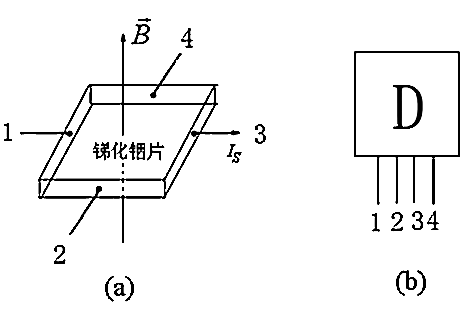
\includegraphics[width=0.8\linewidth]{./img/Fig.1.png}
    \caption{Indium antimonide sheet and its package}
    \label{fig:figure1}
  \end{figure}

  In this experiment, we use an indium antimonide sheet as shown in Figure.1, and create an electromagnetic field of strength $B$, the current is passed through pin 1 and pin 3, and resistance between 1 and 3, 2 and 4 is measured. Due to Hall Effect, pin 2 and pin 4 could be considered a battery with resistance inside, the measurements are done by the following methods:

  \begin{figure}[H]
    \centering
    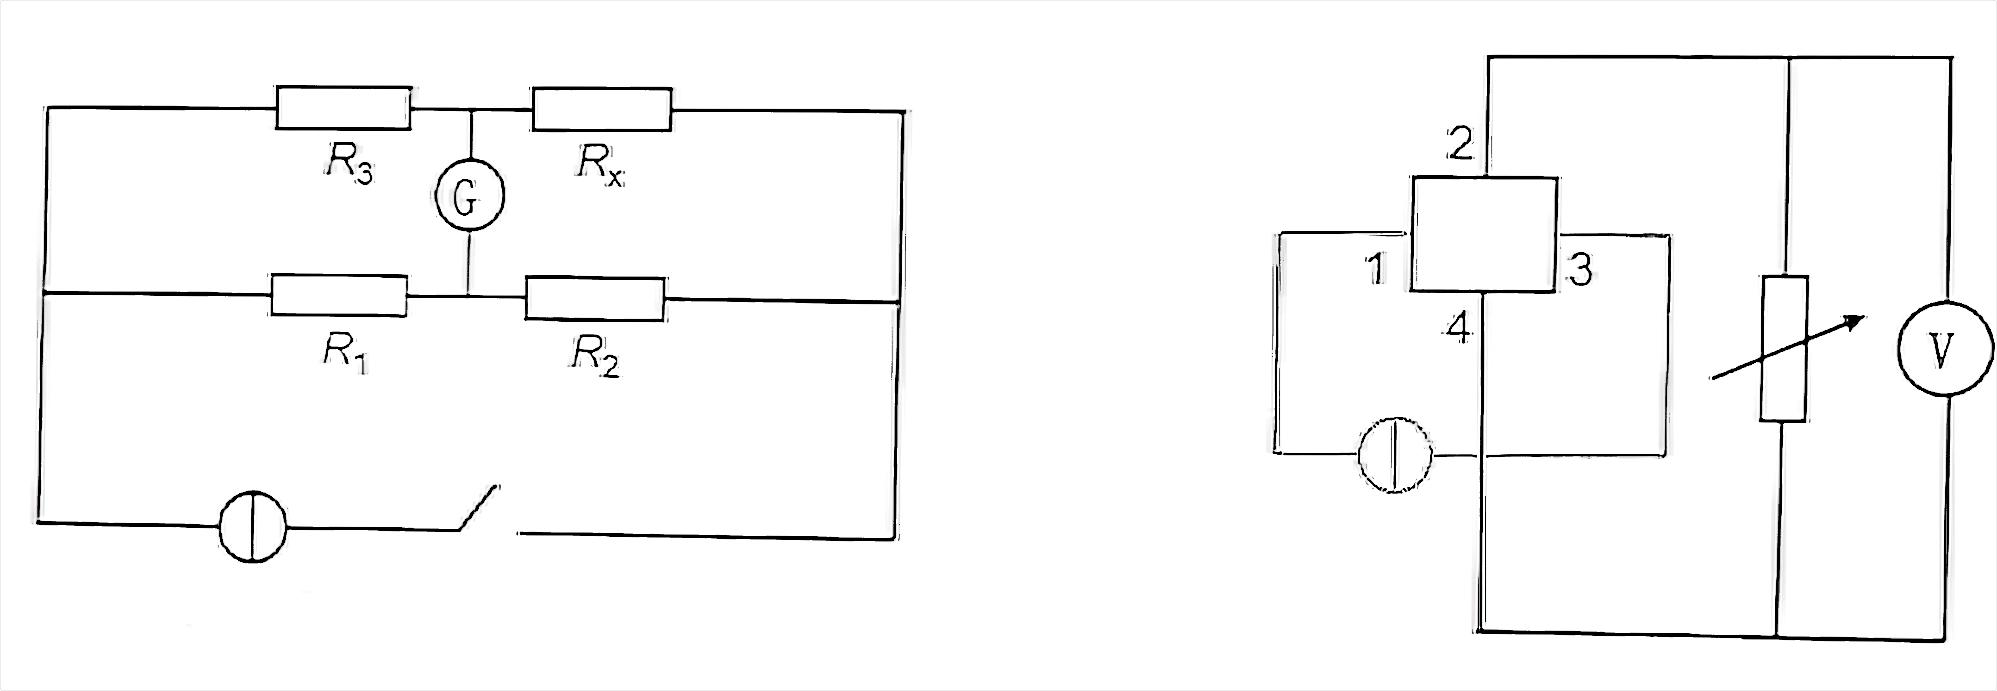
\includegraphics[width=0.8\linewidth]{./img/Fig.2.jpg}
    \caption{Circuits used to measure resistance}
    \label{fig:figure2}
  \end{figure}

  To measure resistance between 1 and 3, a balanced electrical bridge is used to give higher precision results, as shown in Figure.2A. Measuring between 2 and 4 is equivalent to measuring the internal resistance of a battery, as shown in Figure.2B.

  A solenoid is used to provide given magnetic induction intensity $B$, which performance could be expressed in the following equation:

  \begin{equation}
    B = k I,\ \ k = 3500Gs/A
  \end{equation}

  Instrument limitations:

  \begin{equation}
    \left\{
    \begin{aligned}
      I_{coils}  & \leq 1 A  \\
      I_{indium} & \leq 3 mA \\
    \end{aligned}
    \right.
  \end{equation}

  \section*{Materials}
  Connect the circuit with pin 1 and pin 3 connected in Figure.2A, maintain pin 2 and pin 4 disconnected, and later repeat the experiment with pin 2 and pin 4 connected.
  \par
  Starting from $0 mA$, the current to support the coils is increased by $40mA$ each time(up to $800mA$), and the resistance and the current of the coils' power source are recorded.

  Reconnect the circuit as shown in Figure.2B, and repeat the experiment with the same current steps. Notice that this time we need to adjust the resistor $R$ in Figure.2B to the following values: $100\Omega, 200\Omega, 300\Omega,400\Omega$ and record the voltage $V$ and current $I$.

  \section*{Results}
  Results and images are attached in a separate paper.
  \section*{Discussion}
  As shown in the image Figure.3, the $\Delta R/R_0 \sim B$ relationship follows:
  \par
  When B is small, $\Delta R/R_0 \propto B^2$;
  when B is large, $\Delta R/R_0 \propto B$.

  The resistance between 2\&4 is shown in Figure.4, keeping a roughly linear relationship at its center.
  \section*{References}
  \textit{Most contents were translated from the handout.}
  \newpage
\end{multicols*}
\section*{Images}
\begin{figure}[H]
  \centering
  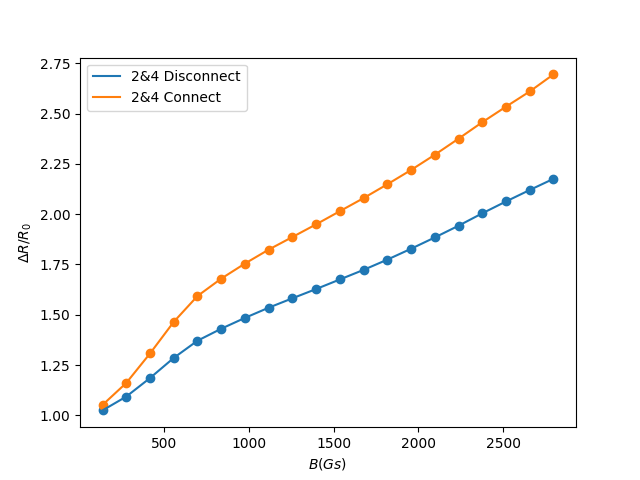
\includegraphics[width=0.6\linewidth]{./img/Fig.3.png}
  \caption{Resistance between 1\&3 with 2\&4 connected/disconnected}
  \label{fig:figure3}
\end{figure}
\begin{figure}[H]
  \centering
  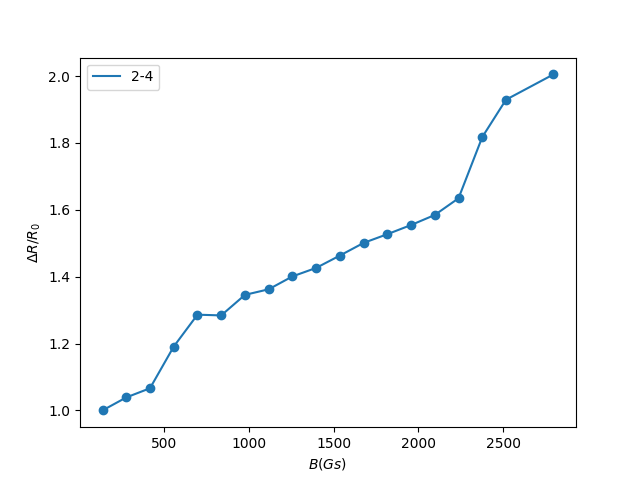
\includegraphics[width=0.6\linewidth]{./img/Fig.4.png}
  \caption{Resistance between 2\&4}
  \label{fig:figure4}
\end{figure}
\end{document}